\documentclass[a4paper, 12pt]{mcshw}
\begin{document}
	\Letsmaketitle{2}
    \begin{enumerate}
        \item 
        How does the volume of a sphere of radius two behave as the dimension of the space increases? What if the radius was larger than two but a constant independent of $d$? What function of d would the radius need to be for a sphere of radius $r$ to have approximately constant volume as the dimension increases?

        \textbf{Solution:} 
        \begin{enumerate}
            \item
            $$
            V(d,r)=\frac{2}{d}\frac{\pi^{\frac{d}{2}}}{\Gamma{\frac{d}{2}}}r^d
            $$

            \[
            \frac{V(d,r)}{V(d-2,r)}=\frac{(d-2)\sqrt{\pi}\Gamma(\frac{d-2}{2})r^2}{d\Gamma(\frac{d}{2})},\text{for } d \geq 3
            \]

            for $d = 2k, k \geq 2$,
            $$
            \frac{V(d,r)}{V(d-2,r)}=\frac{(k-1)\pi\Gamma(k-1)}{k\Gamma(k)}=\frac{\pi r^2}{k}
            $$

            for $d = 2k + 1, k \geq 1$,
            $$
            \frac{V(d)}{V(d-2)}=\frac{(2k-1)\pi\Gamma(\frac{2k-1}{2})}{(2k+1)\Gamma(\frac{2k+1}{2})}=\frac{2\pi{r}^2}{2k+1}
            $$
            As we can see, for $d=2k$, $\frac{V(d, r)}{V(d-2,r)}$ goes decreasingly from value greater than 1 to value less than 1, so does the behaviour for $d=2k+1$. And the two threshold are $k=\pi{r}^2$ and $k=\pi{r}^2+\frac{1}{2}$, so close to each other. So generally we can say, for $r \geq 2$, the volume of the sphere goes up, and then goes down.

            \begin{center}
                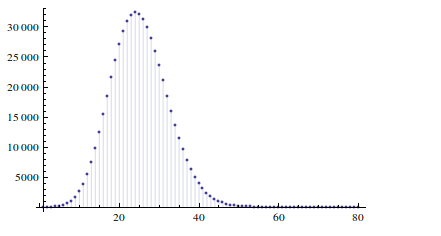
\includegraphics[height=5cm]{1.png}

                \vspace{-4mm}\scriptsize{$r=2$}
            \end{center}

            \begin{center}
                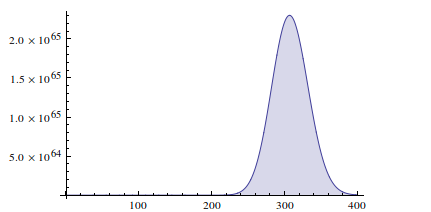
\includegraphics[height=5cm]{2.png}

                \vspace{-1mm}\scriptsize{$r=7$}
            \end{center}
            \item
            It requires that 
            $$
            V(d,r)=\frac{2}{d}\frac{\pi^{\frac{d}{2}}}{\Gamma{\frac{d}{2}}}r^d\approx Constant
            $$
            then
            $$
            r\approx {(Constant\frac{\Gamma(\frac{d}{2})d}{2\pi^{\frac{d}{2}}})}^{\frac{1}{d}}\approx{(Constant\frac{\Gamma(\frac{d}{2}+1)}{\pi^{\frac{d}{2}}})}^{\frac{1}{d}}
            $$
            And we use the Stirling's approximation the simplify the fomula
            $$
            r\approx C^{\frac{1}{d}}\frac{d^{\frac{1+d}{2d}}}{\sqrt{2\pi e}}
            $$
            where $C$ can be any positive real number
            \begin{center}
                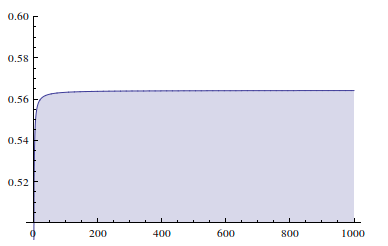
\includegraphics[height=5cm]{3.png}

                \vspace{-3mm}\scriptsize{$C=1$}
            \end{center}
        \end{enumerate}

        \item Consider the upper hemisphere of a unit-radius sphere in d-dimensions. What is the height of the maximum volume cylinder that can be placed entirely inside the hemisphere? As you increase the height of the cylinder, you need to reduce the cylinder's radius so that it will lie entirely within the hemisphere.

        \textbf{Solution:} Let $r$ be the radius of the cylinder, $0 \leq r \leq 1$.
        then the height is
        $$
        \sqrt{1-r^2}
        $$
        now we can calculate the volume
        $$
        V(r)=V(d-1)r^{d-1}\sqrt{1-r^2}
        $$
        then we differentiate it
        $$
        \frac{dV(r)}{dr}=V(d-1)\Big((d-1)r^{d-2}\sqrt{1-r^2}-\frac{r^d}{\sqrt{1-r^2}}\Big)
        $$
        if we let it equals 0, we get
        $$
        r=\sqrt{\frac{d-1}{d}} 
        $$
        $$
        h=\frac{1}{\sqrt{d}}
        $$
        
    \end{enumerate}
\end{document}
